\documentclass{article}

\usepackage{graphicx}
\usepackage{mathtools}
\usepackage{amsmath,amsthm,amssymb}
\DeclarePairedDelimiter{\ceil}{\lceil}{\rceil}
\DeclarePairedDelimiter{\floor}{\lfloor}{\rfloor}
\usepackage{multicol}
\usepackage[skip=3pt]{caption}
\usepackage[top=1in, bottom=1in, left=1in, right=1in]{geometry}
\usepackage{subcaption}
\usepackage{fancyhdr}
\usepackage{tabulary}
\usepackage{times}
\usepackage{titling}
\usepackage{datetime}
%\pagestyle{fancy}
\usepackage[most]{tcolorbox}
\usepackage[T1]{fontenc}
\usepackage[font=small,labelfont=bf,tableposition=top]{caption}
\DeclareCaptionLabelFormat{andtable}{#1~#2  \&  \tablename~\thetable}
\usepackage{slashbox}
\usepackage{algorithm}
\usepackage{algpseudocode}
\algnewcommand\algorithmicforeach{\textbf{for each}}
\algdef{S}[FOR]{ForEach}[1]{\algorithmicforeach\ #1\ \algorithmicdo}

\newcommand{\tab}[1][1]{\noindent \hspace{#1cm} }

\usepackage[style=numeric]{biblatex}
\bibliography{myreferences.bib}

\begin{document}

\section*{} % HEADER
\noindent \textbf{CSCE 586 - Design and Analysis of Algorithms}

\noindent \textbf{Date:}  \today 

\noindent \textbf{Name:}  Micah Hayden

\noindent \textbf{Assignment:}  Homework \#4

\noindent \textbf{Documentation:} None 

\hrulefill


\section*{Chapter 7, Problem \#19 Part a}

\subsection*{Problem Statement:}  
Give a polynomial-time algorithm that takes the numbers $p_1, p_2, ...,p_n$, and the lists $L_1, ..., L_k$, and does the following two things.
\begin{itemize}
	\item Return lists $L'_1, L'_2, ..., L'_k$ satisfying properties (A) and (B); or
	\item Report (correctly) that there is no set of lists $L'_1, L'_2, ..., L'_k$ that satisfies both properties (A) and (B).
\end{itemize}

\subsection*{Description of Algorithm:}
This algorithm utilizes the Ford-Fulkerson algorithm to create a schedule of doctors given the constraints (A) and (B) \cite{algDesign}.

\begin{figure}[h!]
	\label{Fig_19a}
	\centering
	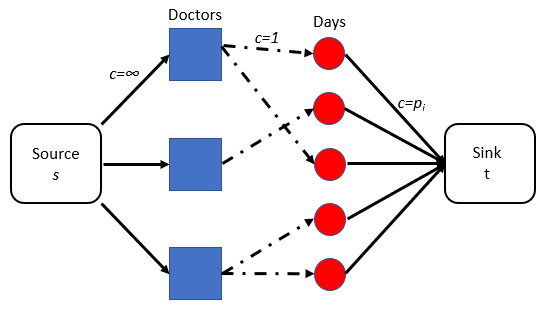
\includegraphics[scale=.75]{Images/19a_Flow.png}
	\caption*{
	\centering
	\footnotesize }
	\caption{Graphical Representation of Scheduling Problem}
\end{figure}

Edges from the source to each doctor have capacity, $c=\infty$; edges from doctors to days have capacity, $c = 1$; and edges from days to the sink $t$ have capacity, $c=p_i$.

The only difference to the traditional Ford-Fulkerson algorithm is the final check to verify the validity of the result.  If the solution is a valid scheduling, the algorithm then loops through the resulting paths and creates the output lists $L'$ for each doctor $j$.

\newpage 
\begin{algorithm}
\caption{Max-Flow - Doctor Scheduling}
\label{alg1}
\begin{algorithmic}
\State Initially $f(e)=0$ for all $e$ in $G$
\While {there is an $s-t$ path in the residual graph $G_f$}
	\State Let $P$ be a simple $s-t$ path in $G_f$
	\State $f' = augment(f, P)$
	\State Update $f$ to be $f'$
	\State Update the residual graph $G_f$ to be $G_{f'}$
\EndWhile
\State Let $ A  = G_f - {t}$, and $B = {t}$.
\If {Cut ($A$, $B$) is \textbf{not} a minimum cut in $G_f$}
	\State \Return There exists no set of lists $L'_1, L'_2, ..., L'_k$ satisfying both properties (A) and (B).
\Else
	\For {day $i$, $i \leq n$ } 
		\State Append Day $i$ to $L'_j$ if there is a path $(i, j)$ in $G_f$
	\EndFor
\EndIf
\State \Return Lists $L'_1, L'_2, ..., L'_k$
\end{algorithmic}
\end{algorithm}

\vspace{-.5cm}
\subsection*{Proof:}
\noindent \textbf{Algorithm correctly identifies if there is not a valid set of lists:}
\newline If there exists a satisfactory set of lists $L'_1, ..., L'_k$, then the flow into the sink $t$ has value: $f_{max} = \sum_{i = 1}^n p_i$.  The capacity from each day $i$ to the sink $t$ has value $c_i = p_i$.  If the value of the min cut/max flow has the expected value, there was a satisfactory set of lists; otherwise, there is not.  This algorithm, as a direct adaptation of the Ford-Fulkerson algorithm, produces a maximum flow by \textbf{7.10} \cite{algDesign}.

\noindent \textbf{Property A:} Doctor $j$ only works on days he or she finds acceptable. \newline
In graph $G$, there are only paths from doctor $j$ to days $i$ which he or she finds acceptable.  Thus, there is no flow $f$ which includes any non-acceptable days.

\noindent \textbf{Property B:}  There are exactly $p_i$ doctors at work on day $i$ \newline
The capacity out of any day $i$ has $c_i = p_i$, for all $i$.  To be an acceptable solution, the maximum flow, $f$, must equal the sum of the capacities $p_i$ for all days $i$.  This indicates that all days have exactly $p_i$ doctors at work.  Assume there was a day $a$ on which there were less than $p_a$ doctors.  Because the maximum flow $f' < f$, it would not be an acceptable solution.  Assume there is a day $b$ on which there are more than $p_b$ doctors.  Because the capacity of edge $c_{(b, t)} = p_b$, no flow $f'$ can have $f' > f$.  Thus, the only valid, possible solution places exactly $p_i$ doctors on day $i$.

\noindent \textbf{Termination:}  Because all capacities are integers, and each iteration of the Ford-Fulkerson algorithm increases the total flow by some $k \geq 1$, the algorithm will terminate.  Because the maximum flow $f_{max}= \sum_{i=1}^n p_i$, the number of iterations $k'$ must satisfy $k' \leq f_{max}$.

\subsection*{Asymptotic Analysis:}
\noindent \textbf{Worst Case:}
The worst case implementation of a graph $G$ with $m$ edges, and a maximum flow $C$, occurs in $O(mC)$ time.  There is at most an additional $C$ operations (the maximum flow consists of $C$ doctor-day paths, which must each be appended to an output list $L_k$.  Thus, the total run-time would be $O(mC) + O(C) = O(mC)$.
The worst-case input model would be one which can only augment by $1$ with each iteration.  This would result in the run-time stated above $O(mC)$.  If there is no valid set of lists to satisfy the problem's requirements, it will still have a run time of $O(mC)$, but $C < \sum_{i = 1}^n p_i$.
 
\noindent \textbf{Best Case:}
By using the Ford-Fulkerson, and its respective $augment$ operation, each iteration increases the flow by the bottleneck capacity of the $s-t$ path.  Because all edges from doctors to days have a capacity of 1, each iteration will increase the flow by 1.  If there is a valid set of lists, the best case input model will have the same worst-case run time as the worst case input model, $O(mC)$.  
  
\noindent \textbf{Average Case:}
Because the best case and worst case input models produce the same run time, the average case input model will be the same.  Due to the constraints given, the flow will increase by 1 each iteration.

\noindent \textbf{Difficulty:}  3, 
\textbf{Time:}  60 Minutes

\newpage

\section*{Chapter 7, Problem \#19 Part b}

\subsection*{Problem Statement:}  
Describe a polynomial-time algorithm that implements the revised system.  It should take the numbers $p_1, p_2, ..., p_n$, the lists $L_1, ..., L_k$, and the parameter $c > 0$, and do one of the following two things:

\begin{itemize}
	\item Return lists $L'_1, L'_2, ..., L'_k$ satisfying properties (A*) and (B); or
	\item Report (correctly) that there is no set of lists $L'_1, L'_2, ..., L'_k$ that satisfies both properties (A*) and (B).
\end{itemize}

\subsection*{Description of Algorithm:}
This problem utilizes Algorithm \ref{alg1} from Problem \#19 Part A.  However, each doctor has a corresponding gadget node.  This gadget node has a $c_{in} = c$, on the node connecting it to its respective doctor $j$.  The gadget node has an edge to every day $i$ not in $L_j$, with capacity $c_{out}=1$.  The graphical structure is shown in Figure \#2.

\begin{figure}[h!]
	\label{Fig_19b}
	\centering
	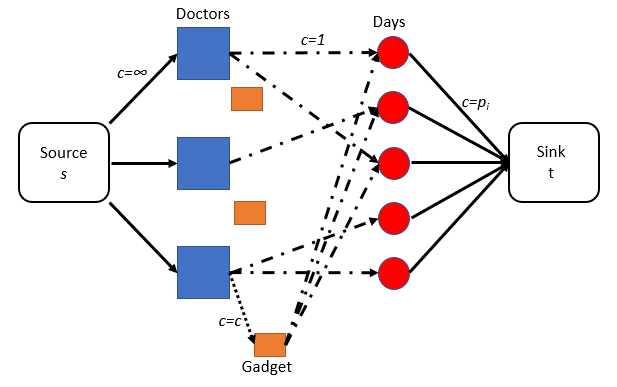
\includegraphics[scale=.6]{Images/19b_Flow.png}
	\caption*{
	\centering
	\footnotesize }
	\caption{Doctor Scheduling with Gadget}
\end{figure}
\subsection*{Proof:}
Problem \#19, Part A proved that the algorithm terminates, that it produces a maximum flow, and that if the maximum flow $f_{max} = \sum_{i=1}^n p_i$, then it returns a set of satisfactory lists, otherwise it returns that there is no such set of lists.  Thus, the only additional proof needed is that it satisfies property $A*$: each doctor, $j$, works no more than $c$ days not included in $L_j$.  

\noindent \textbf{Proof of $A*$:}  Each doctor $j$ has a direct edge to any day $i$ included in $L_j$.  To reach any other days, the flow must go through $j$, into its respective gadget $g_j$, and then to some day $k \notin L_j$.  The capacity of the edge connecting $j$ to $g_j$ has capacity, $c$.  The total flow out of $j$, $f_j \leq c + |L_j|$, $|L_j| $ corresponds to days which doctor $j$ wanted to work.  Thus, the amount of flow from doctor $j$ to non-desired days, must have $f'_j = f_j - |L_j| \leq c$.  Because each doctor has their own gadget, this concludes that no doctor $j$ works more than $c$ days not in $L_j$.

\subsection*{Asymptotic Analysis:}
\noindent \textbf{Worst Case, Best case, average case:} The only change from Part A is the introduction of the gadget node for each doctor. Because this has no effect on the maximum flow of the network (sum of $p_i$ for all $i$), the asymptotic analysis for the worst, best, and average cases are identical to those of Problem \#19 Part A, and is $O(mC)$.

\noindent \textbf{Difficulty:}  2, \textbf{Time:}  30 Minutes

\newpage

\section*{Chapter 8, Problem \#2}

\subsection*{Problem Statement:}  
Define the Diverse Subset Problem as follows:  Given an $m \times n$ array $A$ as defined above, and a number $k \geq m$, is there a subset of at least $k$ of customers that is $diverse?$.
Show that Diverse Subset is NP-complete.

\subsection*{Proof:}
Let $Y$ be the Diverse Subset problem.

\noindent \textbf{Show that $Y \in NP$:} \newline
$Y$ is \textbf{NP} because there exists some certifier $t$.  
Given a set $S$ of customers, with $|S| \leq k \leq m$, $t$ can certify that $S$ is diverse by checking if any items bought by $x \in S$ have been purchased by any previous customer $x' \in S$.

\noindent \textbf{Choose an NP-Complete Problem $X$:}  Let $X$ be the Independent Set.

\noindent \textbf{Prove that $X \leq_P Y$:}

Consider the following matrix $A$:

\begin{table}[h!]
\begin{center}
\begin{tabular}{|c||*{4}{c|}} \hline
\backslashbox{Customer}{Item}
&\makebox[3em]{\#1}&\makebox[3em]{\#2}&\makebox[3em]{\#3}
&\makebox[3em]{\#4} \\ \hline \hline
A & 0 & 1 & 1 & 1 \\ \hline
B & 1 & 0 & 0 & 0 \\ \hline
C & 0 & 1 & 0 & 1 \\ \hline
\end{tabular}
\caption{Matrix $A$}
\end{center}
\end{table}

\noindent First, create a graph $G(V,E)$ such that there is a vertex for each customer, and a node for each item the customer buys.  Each customer $s$ has an edge to each item $i$ that they purchase.  Next, add an edge connecting duplicate items.  These edges correspond to conflicts because $x \geq 2$ customers bought that particular item.  Figure \#3 shows $G$.

\begin{figure}[!h]
  \centering
  \begin{minipage}[b]{0.45\textwidth}
    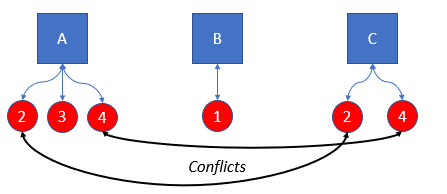
\includegraphics[width=.9\textwidth]{Images/Discrete_Init.png}
    \caption{$G$ - Initial representation of Matrix $A$}
  \end{minipage}
  \hfill
  \begin{minipage}[b]{0.45\textwidth}
    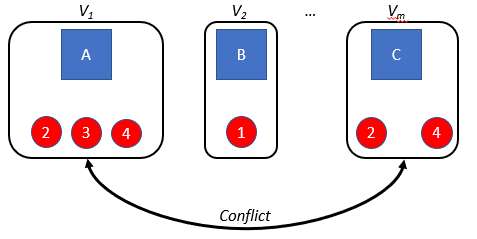
\includegraphics[width=.9\textwidth]{Images/Discrete_Final.png}
    \caption{$G'$ - Final representation of Matrix $A$}
  \end{minipage}
\end{figure}

Transform $G$ into $G'$ by replacing each customer/item set with a single vertex $V_1, V_2, \dots , V_m$.  Let the set of these vertices be $V$.
If there were any conflicts in $G$, $G'$ has a corresponding conflict; however, if $x \geq 2$ conflict edges connect two vertices, replace them with a single edge.  Figure \#4 shows $G'$, generalized to extend to $V_m$.

To create a diverse subset from $G'$, simply choose a set $S \subset V$, such that $S$ is an independent set.  Because each vertex in $V$ has a single customer node, the diverse subset of customers is simply each customer node, $c \in S$.
Thus, Independent Set $\leq_P$ Diverse Subset.
Because the Independent-Set problem is \textbf{NP-Complete} by \textbf{8.16} \cite{algDesign}, 
The Diverse Subset problem is thus \textbf{NP-Complete} by \textbf{8.14}.

\noindent \textbf{Difficulty:}  4

\noindent \textbf{Time:}  45 Minutes

\newpage

\section*{Chapter 8, Problem \#28}

\subsection*{Problem Statement:}  
Prove that the Strongly Independent Set Problem is NP-complete.

\subsection*{Proof:}
Let $Y$ be the Strongly Independent Set problem.

\noindent \textbf{Show that $Y \in NP$:} \newline
$Y$ is \textbf{NP} because there exists some certifier $t$.  
Given a set $I$ nodes, with $|I| \geq k$, $t$ can certify that $I$ is strongly independent by iterating through the nodes of $I$ and marking each adjacent node $y$ as visited.  If it encounters an adjacent node $y'$ that has been visited, it must have been visited from some earlier node $x \in I$.  If it encounters no duplicate adjacent nodes, it is strongly independent.

\noindent \textbf{Choose an NP-Complete Problem $X$:}  Let $X$ be the Independent Set problem.

Independent Set is \textbf{NP-Complete} by \textbf{8.16} \cite{algDesign}.

\noindent \textbf{Prove that $X \leq_P Y$:}

Consider a graph $G(V, E)$, and a set $I \subset V$.
Consider two nodes, $u \in I$ and $v \in I$.  If $I$ is an independent set, edge $(u, v) \notin E$. Let there be a path $P$ that connects $u$ to $v$.  If $I$ is a strongly independent set, $|P| \geq 3$.  

In polynomial-time, it is possible to determine whether $I$ is a strongly independent set, if $I$ is known to be an independent set.

Consider graph $G$ in Figure \#5. Nodes 1-4 create an independent set $S$, with $|S|=4$.  
To verify that they create a strongly independent set, create a new graph $G'(V,E)$, where each vertex $V_1, \dots , V_n$ represents a node of the independent set, its adjacent nodes, and its edges.  
Create an edge connecting any vertices $v$ that contain duplicate nodes.  
Figure \#6 shows these edges, representing the conflicts caused by nodes $b$ and $c$.

\begin{figure}[!h]
  \centering
  \begin{minipage}[b]{0.45\textwidth}
    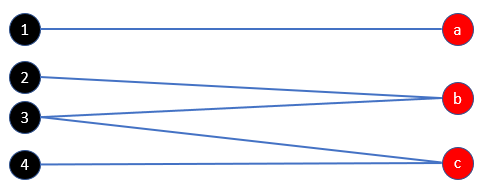
\includegraphics[width=.9\textwidth]{Images/Independent.png}
    \caption{$G$ - Independent Set}
  \end{minipage}
  \hfill
  \begin{minipage}[b]{0.45\textwidth}
    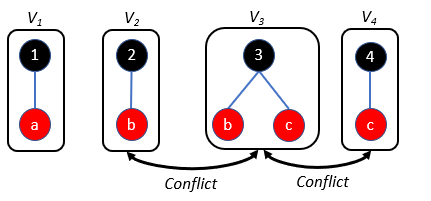
\includegraphics[width=.9\textwidth]{Images/Strong_Independent.png}
    \caption{$G'$ - Modified from $G$}
  \end{minipage}
\end{figure}

\noindent If an Independent Set $S$ is Strongly Independent, there will be no conflicts.  A strongly independent set $S'$ can be found by finding the set of nodes $S' \subset S$, where all elements $e \in S'$ satisfy $e_i \in v_i, e_j \in v_j$, and $(v_i, v_j) \notin E$, for $G'$.

\noindent Thus, Independent Set $\leq_P$ Strongly Independent Set. 
Because the Independent-Set problem is \textbf{NP-Complete} by \textbf{8.16} \cite{algDesign}, 
The Strongly Independent Set problem is \textbf{NP-Complete} by \textbf{8.14} \cite{algDesign}.

\noindent \textbf{Difficulty:}  5

\noindent \textbf{Time:}  45 Minutes

\printbibliography


\end{document}
